% -*- mode:LaTex; mode:visual-line; mode:flyspell; fill-column:75-*-

\chapter{Conclusions} \label{chapConclusions}


\section{Future Work}
Though much effort went into providing an important framework for the haptic to operate smoothly from a hardware standpoint, the most important progress with the final prototype was the solidification of the software framework. With the integration of delay independent state-machines performing synchronous tasks, haptic mode selection, and precise bpm control, the vibrotactile haptic could enter the next phases of development. 

The addition of BLE capability to issue commands over a paired interface such as an app on a smartphone, custom PCB to minimize form factor, and independent node abstraction of each vibrotactile could be realized. This would allow wearers capability to place a programmable array anywhere on their body enabling wide surface area dispersion. 

Lastly, experimentation with other types of vibrotactiles; either the Tactor, TacHammer, or LNA's would be more optimized for touch applications with cleaner signals, dynamic range, and optimized for skin resonance (250Hz).

\subsection{Wireless Prototype}
Over the course of summer of 2018, a wireless prototype was developed which eliminated the FTDI over USB interface and was completely reliant on battery power. A 9 V was connected to a voltage regulator supplying up to 5 V for the motors and 3.3V for the new MCU, sourcing up to 500 mA/hour with enough isolation to have a significantly stronger motor vibration. The MCU was based on the Particle ecosystem, a cloud based IoT framework, and granted BLE and wireless capability. 
\begin{figure}[H]
    \centering
    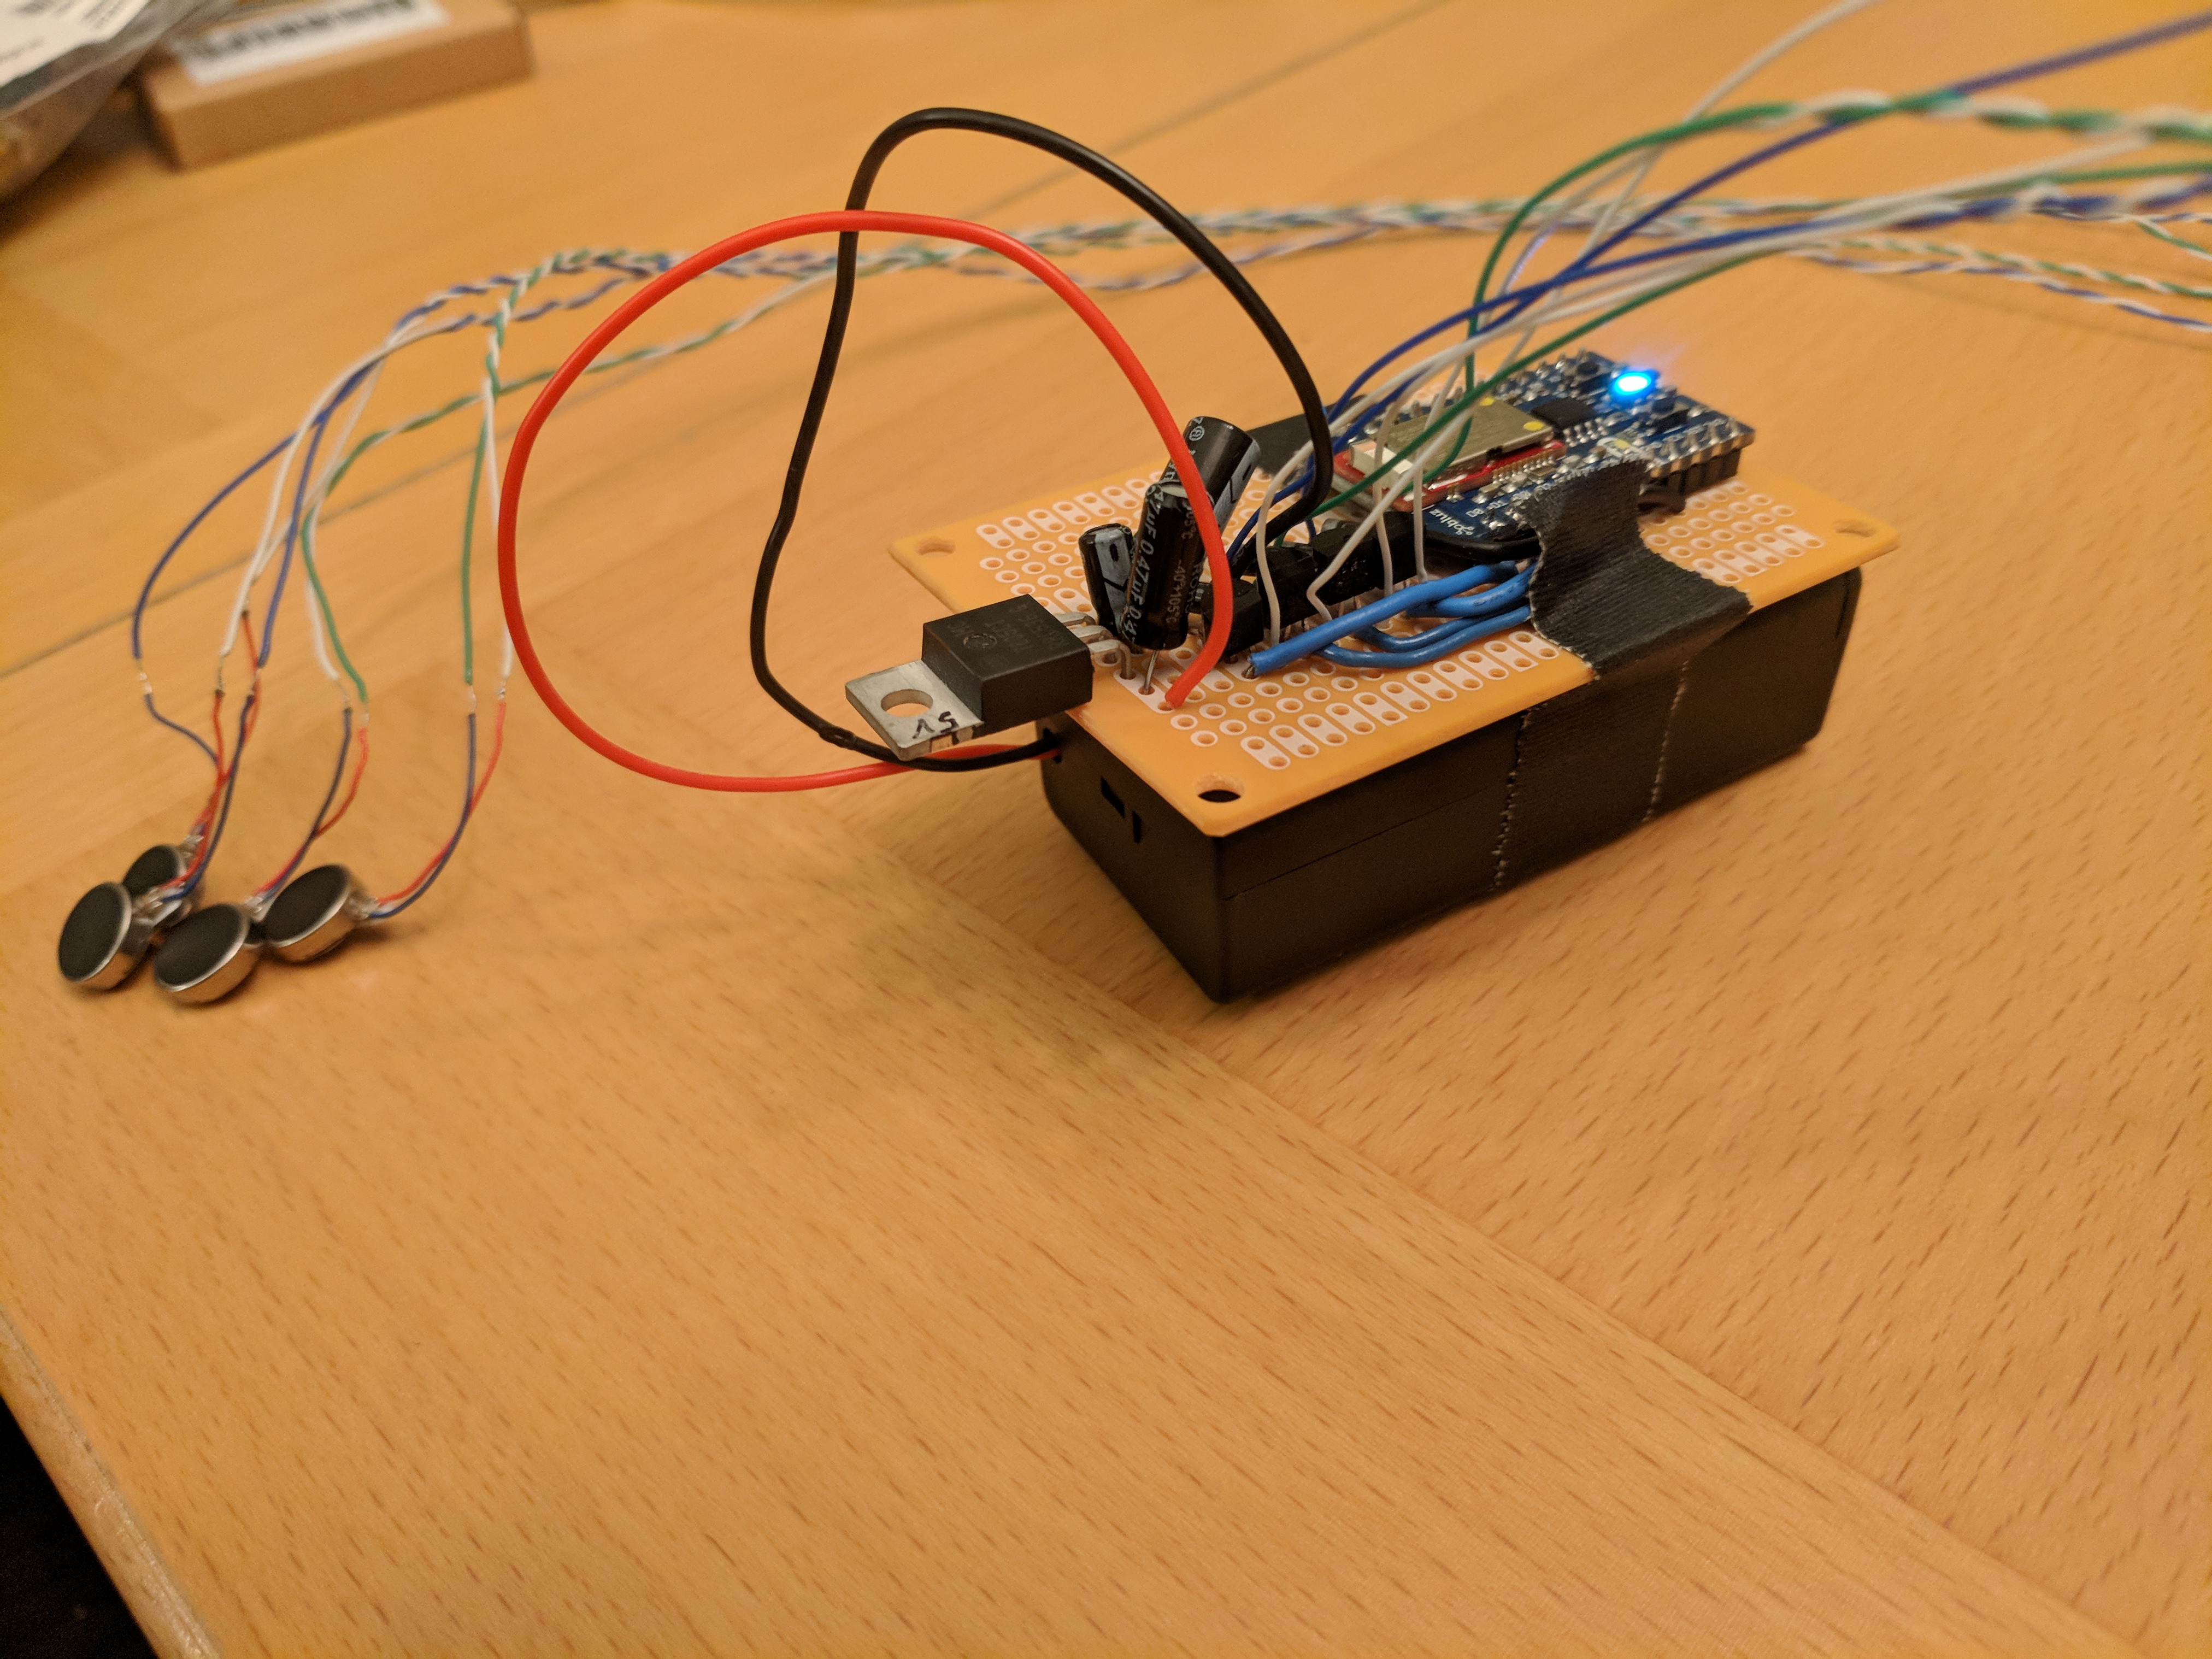
\includegraphics[width=\columnwidth]{latestProto}
    \caption{Latest wireless prototype with cloud capability}
\end{figure}
The code was altered to adapt the publish/subscribe methodology where simple numeric BPM values could be passed as API calls to the device given proper OAuth2 authentication. For example, to start the motor at 60 bpm tempo:
\begin{lstlisting}[language=html]
    curl https://api.particle.io/v1/devices/<deviceID>/motor \
       -d arg="1" \
       -d access_token=<accessToken>

    curl https://api.particle.io/v1/devices/<deviceID>/motor \
       -d arg="60" \
       -d access_token=<accessToken>
\end{lstlisting}

\subsection{Beat Tracking}
As part of the PhD work completed at the Queen Mary University of London, Adam Stark has developed a causal beat tracking algorithm intended for use in live performances\footnote{\url{http://adamstark.co.uk/project/btrack-a-real-time-beat-tracker/}}\ref{stark2009real}.

\subsection{Extra-musical Applications}

Parkingson's research

Stroke gait rehabilitation research \cite{holland2014gait}

Through their research they discovered the extension of the application towards those with restricted mobility and morphed the project into the haptic bracelet 4 years later.

Stroke survivors usually suffer from  for the purpose of gait rehabilitation. The results were promising. 

Paper discusses the prior research of audio stimulation and how it yields immediate improvement through entrainment but that they are not lasting

Focussed on triggering the tibialis anterior which contrasts the principles of entrainment, which would utilize rhythmic beats in any sensory modality, regardless of placement. Also haptic masking from leg-to-floor-impact

One patient who was a veteran mentioned that it put a marching sense back into his mind and helped remind him of that sensation of even walking.
